\documentclass{beamer}

\usepackage{geometry} % Pour passer au format A4
\usepackage{graphicx} % Required for including pictures
\usepackage{float} %

\usepackage{amsmath,amsfonts,amssymb,amsthm}
\usepackage[T1]{fontenc}
\usepackage[english,francais]{babel}
\usepackage[utf8]{inputenc}
\usepackage{lmodern}
\usepackage{eurosym} % signe Euros
\usepackage{verbatim}
\usepackage{multicol}

\usetheme{Warsaw}

\title{Démonstration du Théorème de Pythagore}

\begin{document}

\frame{\titlepage}

\begin{frame}
  \frametitle{Démonstration}
 	\begin{figure}[H]
	  \centering
	  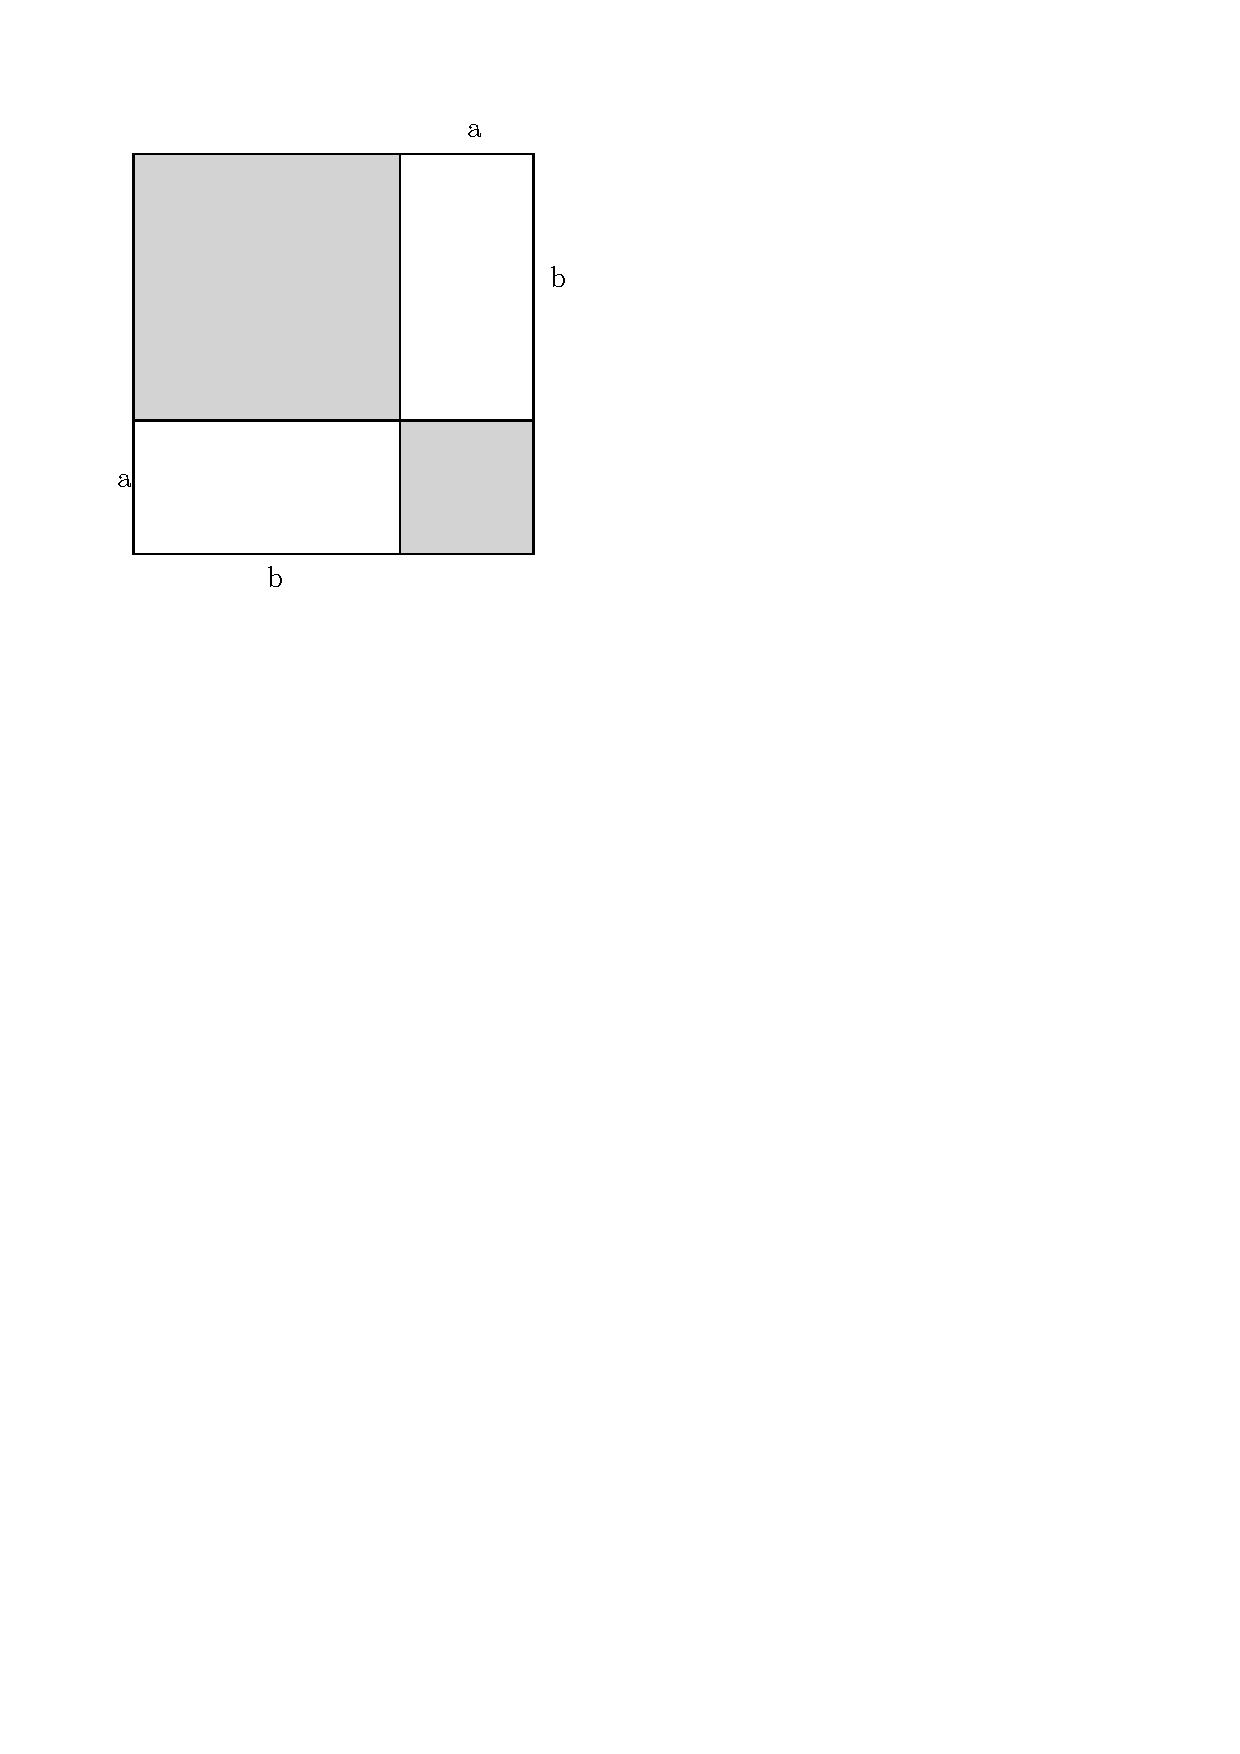
\includegraphics[width=0.65\linewidth]{sources/1/demo-pytha-t0.pdf}
	\end{figure}
\end{frame}

\begin{frame}
  \frametitle{Démonstration}
 	\begin{figure}[H]
	  \centering
	  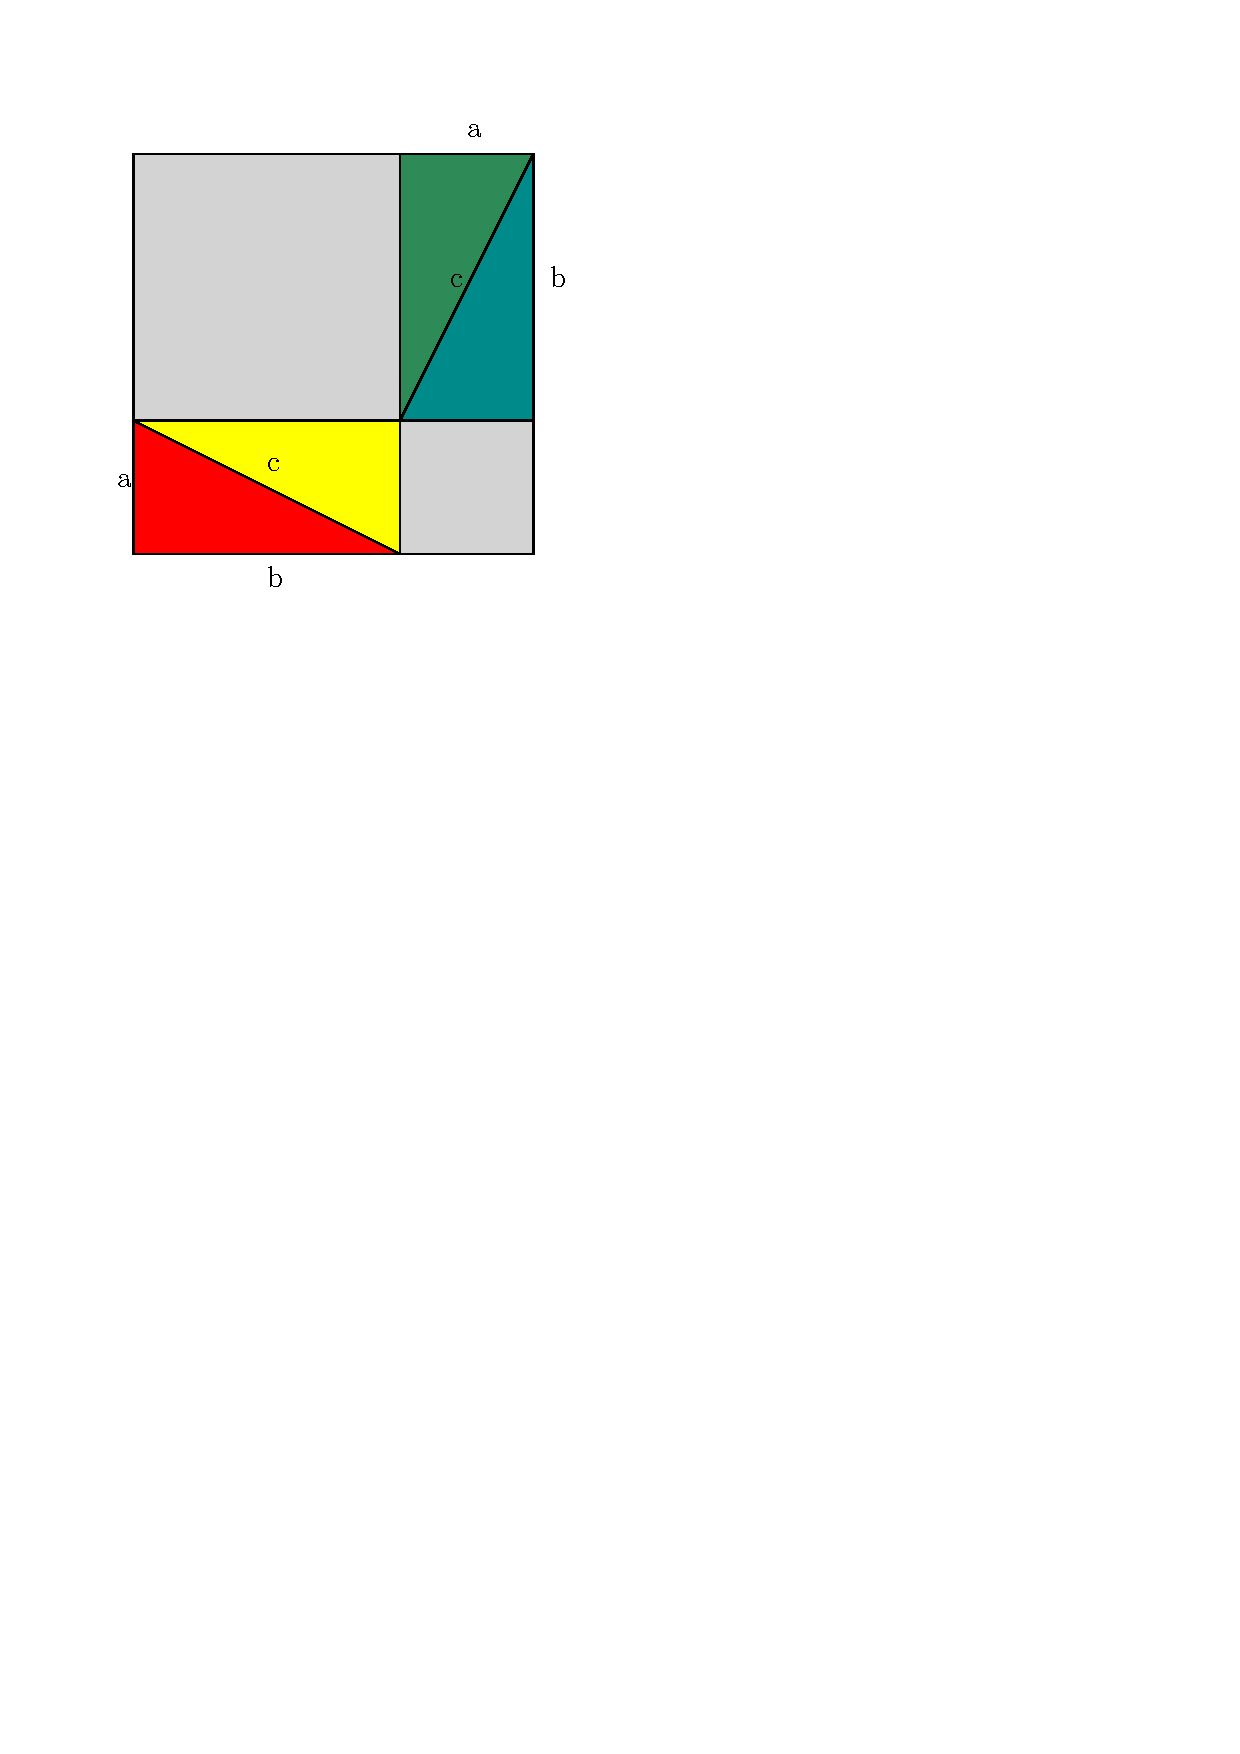
\includegraphics[width=0.65\linewidth]{sources/1/demo-pytha-t1.pdf}
	\end{figure}
\end{frame}

\begin{frame}
  \frametitle{Démonstration}
 	\begin{figure}[H]
	  \centering
	  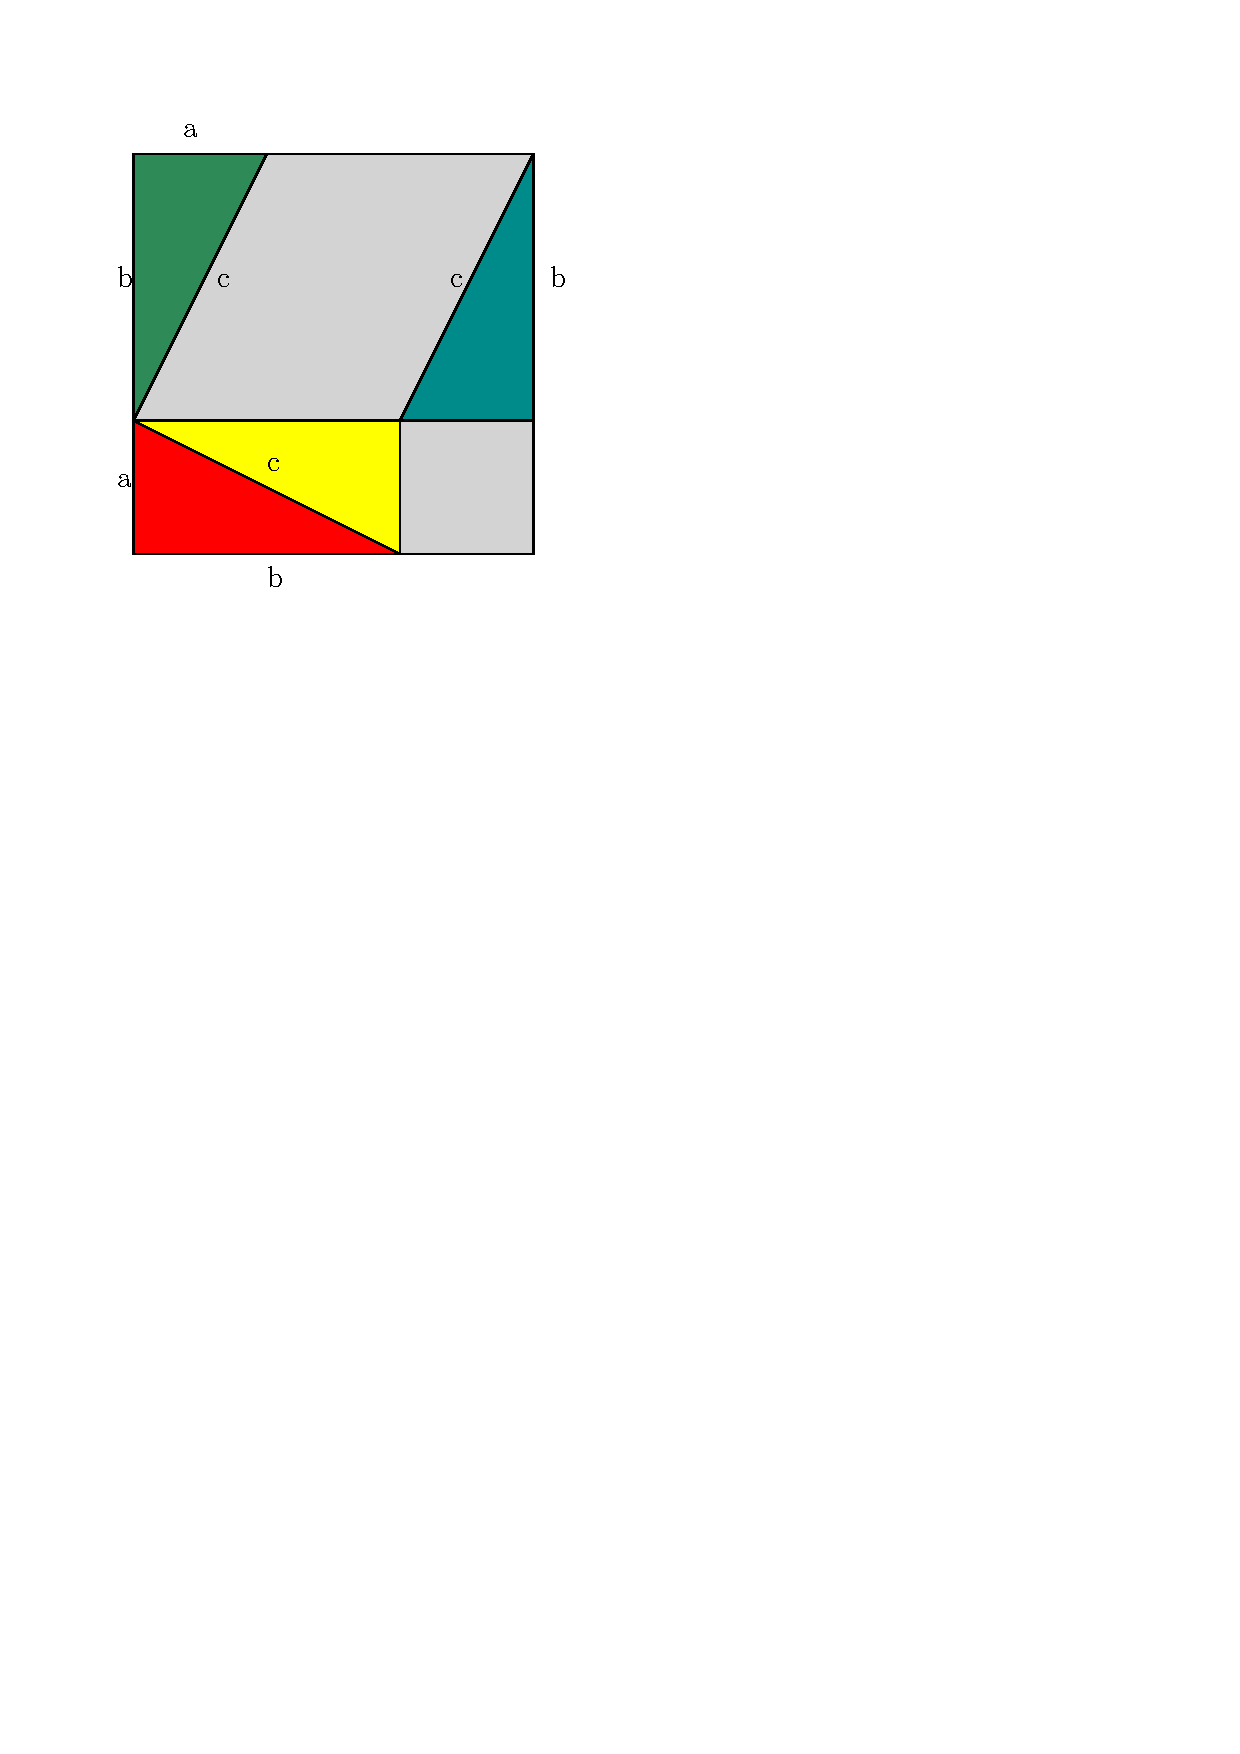
\includegraphics[width=0.65\linewidth]{sources/1/demo-pytha-t2.pdf}
	\end{figure}
\end{frame}
\begin{frame}
  \frametitle{Démonstration}
 	\begin{figure}[H]
	  \centering
	  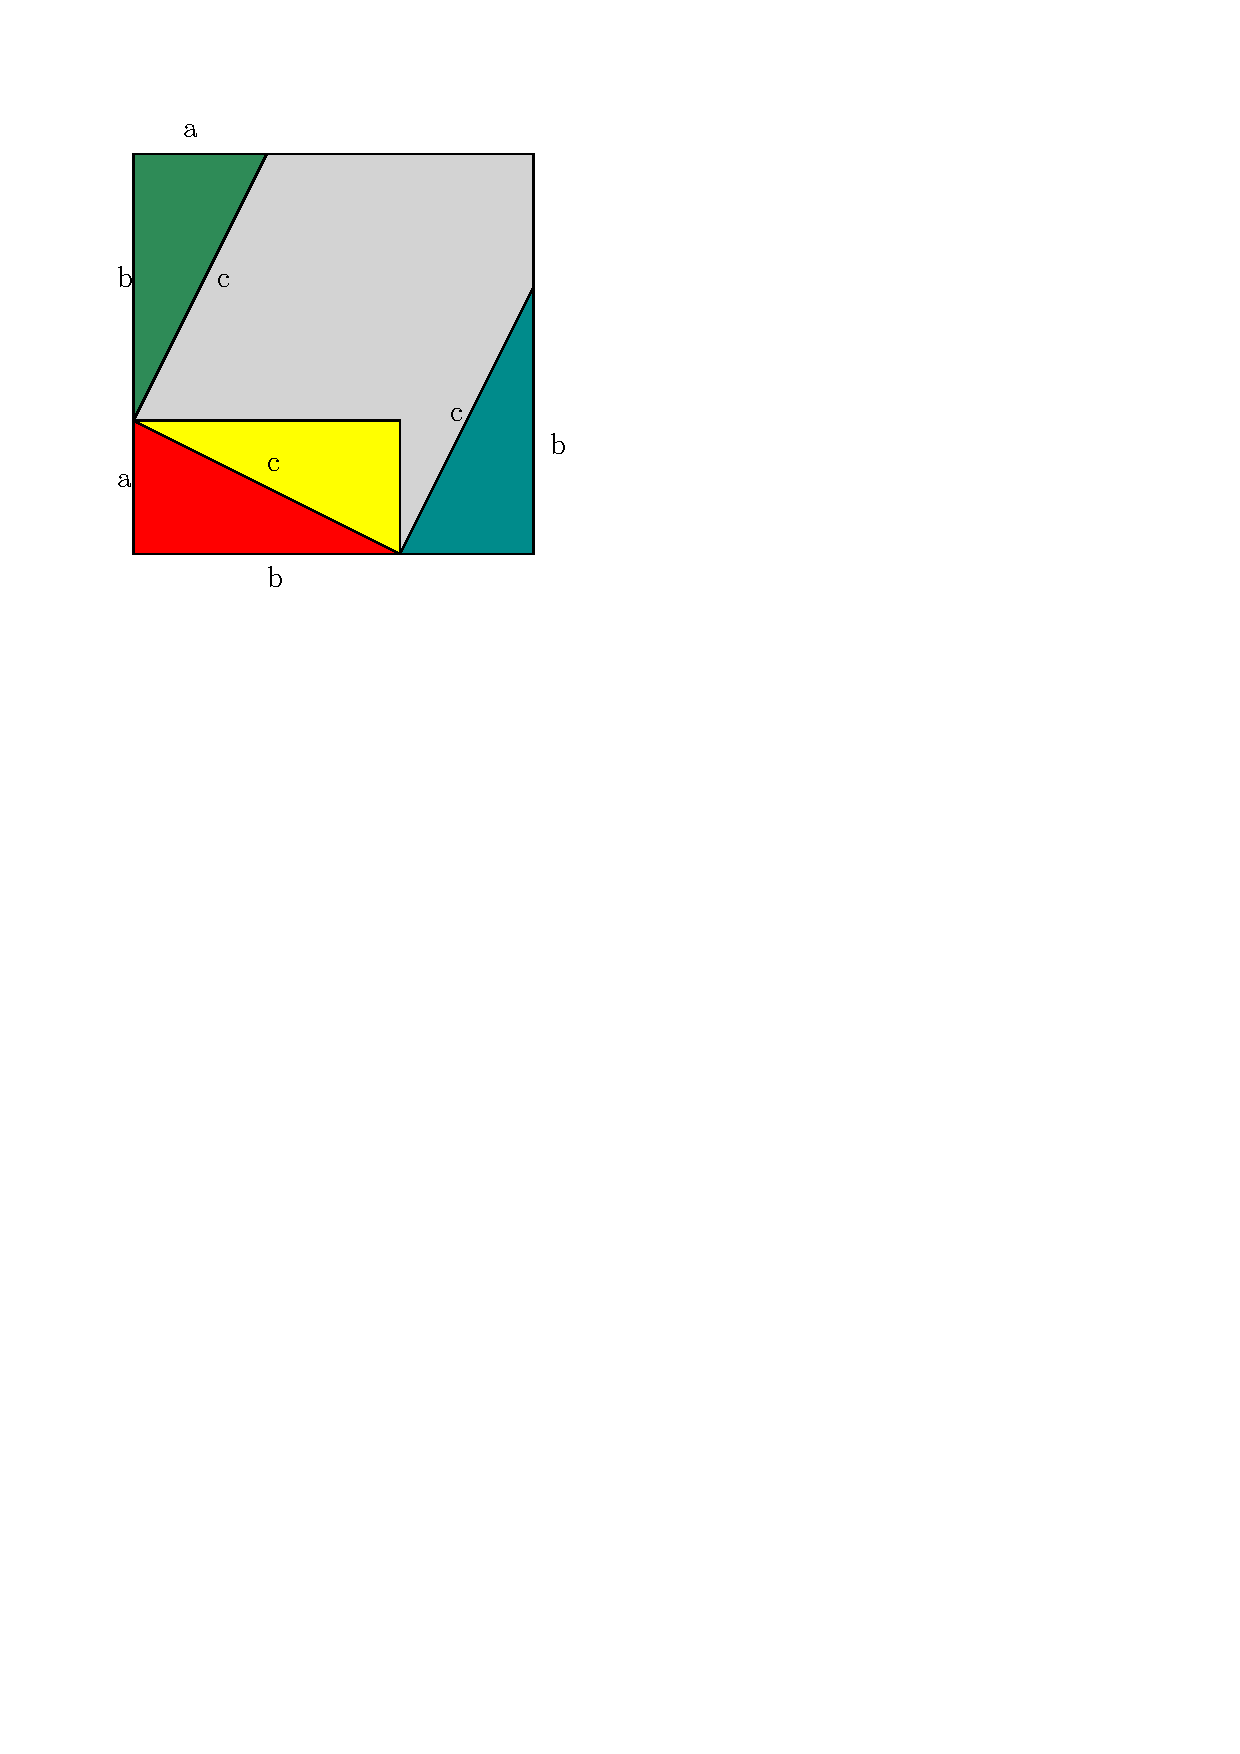
\includegraphics[width=0.65\linewidth]{sources/1/demo-pytha-t3.pdf}
	\end{figure}
\end{frame}

\begin{frame}
  \frametitle{Démonstration}
 	\begin{figure}[H]
	  \centering
	  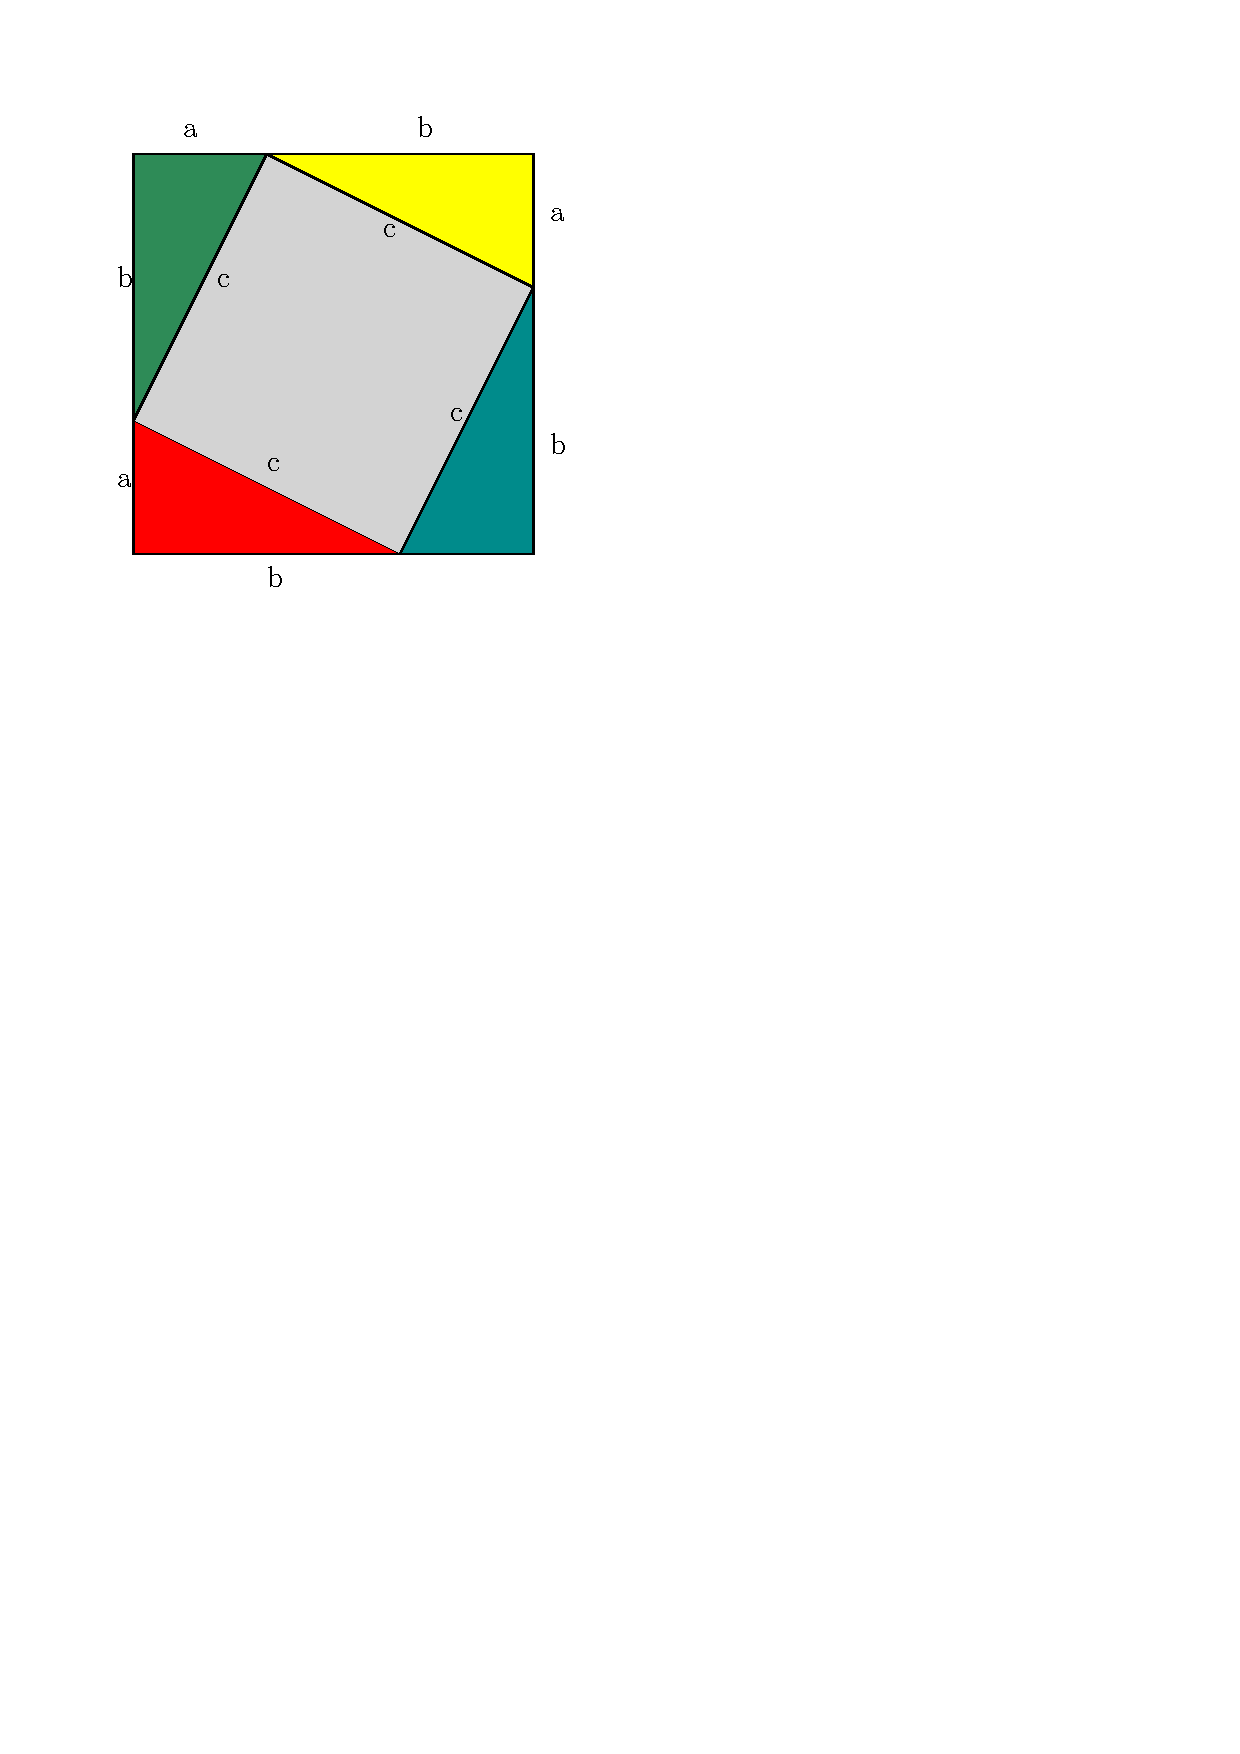
\includegraphics[width=0.65\linewidth]{sources/1/demo-pytha-t4.pdf}
	\end{figure}
\end{frame}

\end{document}
